\documentclass[]{article}
\usepackage{caption,subcaption,graphicx,float,url,amsmath,amssymb,amsthm,tocloft,cancel,thmtools}
\newtheorem{ex}{Exercise}
\newcommand\numberthis{\addtocounter{equation}{1}\tag{\theequation}}

%opening
\title{Chaos}
\author{Simon Crase}

\begin{document}

\maketitle

\begin{abstract}
Miscellaneous calculations  from \cite{ChaosBook}
\end{abstract}

\tableofcontents

\section{Lorenz Equations}

\subsection{Lorenz Equations}
\begin{align*}
	\dot{x} =& \sigma(y-x) \numberthis \label{eq:lorenz:1}\\
	\dot{y} =& \rho x -y - xz \numberthis \label{eq:lorenz:2}\\
	\dot{z} =& xy-bz \numberthis \label{eq:lorenz:3}
\end{align*}
The equilibria are given by
\begin{align*}
	\sigma(y-x) =& 0\\
	\rho x -y - xz  =& 0\\
	xy-bz =& 0
\end{align*}
Assuming $\rho, \sigma, b \ne 0$
\begin{align*}
	y =& x\\
	z =& \frac{xy}{b}
\end{align*}
One solution is $(x,y,z)= (0,0,0)$. The other solution is
\begin{align*}
	\rho x - x-x \frac{x^2}{b} =& 0\\
	\rho -1 - \frac {x^2}{b} =& 0\\
	x^2 =& b(\rho-1)\\
	x =& \pm \sqrt{ b(\rho-1)}\\
	(x,y,z)=& (\pm \sqrt{ b(\rho-1)},\pm \sqrt{ b(\rho-1)},\rho-1)
\end{align*}

\subsection{Pseudo-Lorenz}

Following \cite{miranda1993proto}, we define new variables in \eqref{eq:lorenz:1},  \eqref{eq:lorenz:2}, and \eqref{eq:lorenz:3}.
\begin{align*}
	u =& x^2-y^2 \numberthis \label{eq:miranda:stone:1}\\
	v =& 2 x y \text{, and}\numberthis \label{eq:miranda:stone:2}\\
	N =& \sqrt{u^2+v^2}\\
	=& \sqrt{(x^2-y^2)^2 + 4x^2y^2}\\
	=& \sqrt{x^4 - 2 x^2 y^2 + y^4  + 4x^2y^2}\\
	=& \sqrt{x^4 + 2 x^2 y^2 + y^4}\\
	=& \sqrt{(x^2+y^2)^2}\\
	=& x^2+y^2 \numberthis \label{eq:miranda:stone:N}
\end{align*}

The following identities will be useful.
\begin{align*}
	N+u= & x^2+y^2 + x^2 - y^2 \text{, from \eqref{eq:miranda:stone:1} and \eqref{eq:miranda:stone:N}} \\
	=& 2 x^2 \text{, whence}\\
	x^2 =& \frac{N+u}{2}\numberthis \label{eq:miranda:stone:x}\\
	N - u =& x^2+y^2 - x^2 + y^2 \text{, from\eqref{eq:miranda:stone:2} and \eqref{eq:miranda:stone:N}}\\
	=& 2 y^2 \text{, whence}\\
	y^2 =& \frac{N-u}{2}\numberthis \label{eq:miranda:stone:y}	
\end{align*}

We transform the Lorenz equation to the new coordinates.
\begin{align*}
	\dot{u} =& 2 x \dot{x} - 2 y \dot{y} \text{, from \eqref{eq:miranda:stone:1}}\\
	=& 2x\sigma(y-x)-2y(\rho x - y -xz) \text{, from \eqref{eq:lorenz:1} and \eqref{eq:lorenz:2}}\\
	=&( \sigma - \rho)(2xy) -2\sigma x^2  + 2y^2 + (2xy)z\\
	=& ( \sigma - \rho) v -\sigma (N+u) + (N-u) + vz \text{, using \eqref{eq:miranda:stone:2}, \eqref{eq:miranda:stone:x} and \eqref{eq:miranda:stone:y}}\\ 
	=& ( \sigma - \rho) v + (1-\sigma)N - (1+\sigma)u +vz \numberthis \label{eq:miranda:stone:de:u}\\
	\dot{v} =& 2 \dot{x} y + 2 x \dot{y} \text{, from \eqref{eq:miranda:stone:2}}\\
	=& 2\sigma(y-x)y+2x(\rho x-y-xz)  \text{, from \eqref{eq:lorenz:1} and \eqref{eq:lorenz:2}}\\
	=& 2 \sigma y^2 -2 \sigma x y + 2\rho x^2 -2xy -2 x^2 z\\
	=&  \sigma (N-u) - \sigma v + \rho (N+u) -v - (N+u) z \text{, using \eqref{eq:miranda:stone:2}, \eqref{eq:miranda:stone:x} and \eqref{eq:miranda:stone:y}}\\
	=& (\rho-\sigma) u - (\sigma+1)v + (\rho+\sigma)N - (N+u) z \numberthis \label{eq:miranda:stone:de:v}\\
	\dot{z} =& \frac{1}{2} 2xy - bz \text{, From \eqref{eq:lorenz:3}} \\
	=& \frac{1}{2}v - z \text{, from \eqref{eq:miranda:stone:2}} \numberthis \label{eq:miranda:stone:de:z}
\end{align*}
\section{Homework 2}

\subsection{Homework, Q1.3 Floquet Multipliers}

From \cite[Q1.3]{ChaosBook}
\begin{align*}
	\dot{q} =& p + q\big(1-q^2-p^2\big) \numberthis \label{eq:dot_q}\\
	\dot{p} =&-q + p\big(1-q^2-p^2\big) \numberthis \label{eq:dot_p}
\end{align*}
Transform to polar coordinates
\begin{align*}
	q =& r \cos{\theta}\\
	p =& r \sin{\theta}\\
	\dot{q} =& \dot{r} \cos{\theta}  - r \sin{\theta} \, \dot{\theta} \numberthis \label{eq:dot_q_polar}\\
	\dot{p} =& \dot{r} \sin{\theta}  + r \cos{\theta} \, \dot{\theta} \numberthis \label{eq:dot_p_polar}
\end{align*}
Substituting \eqref{eq:dot_q} and \eqref{eq:dot_p} in \eqref{eq:dot_q_polar} and \eqref{eq:dot_p_polar}
\begin{align*}
	\cos{\theta} \dot{q} + \sin{\theta} \dot{p} =& \dot{r}\cos^2\theta -\cancel{r \cos{\theta} \sin{\theta}\; \dot{\theta}} + \dot{r}\sin^2\theta+ \cancel{r \cos{\theta} \sin{\theta}\; \dot{\theta}}\\
	=& \dot{r}  \numberthis \label{eq:dot_r0}\\
	\sin{\theta} \dot{q} - \cos{\theta}\dot{p} =& \sin{\theta} \big[\cancel{\dot{r} \cos{\theta}}  - r \sin{\theta} \, \dot{\theta}\big] - \cos{\theta}\big[\cancel{\dot{r} \sin{\theta}}  + r \cos{\theta} \, \dot{\theta}\big]\\
	=& - r \big(\cos^2\theta+\sin^2\theta\big) \dot{\theta}\\
	=&-r \dot{\theta} \numberthis \label{eq:dot_theta}
\end{align*}
\begin{figure}[H]
	\caption{From \eqref{eq:dot_theta} the solution circles clockwise.}
	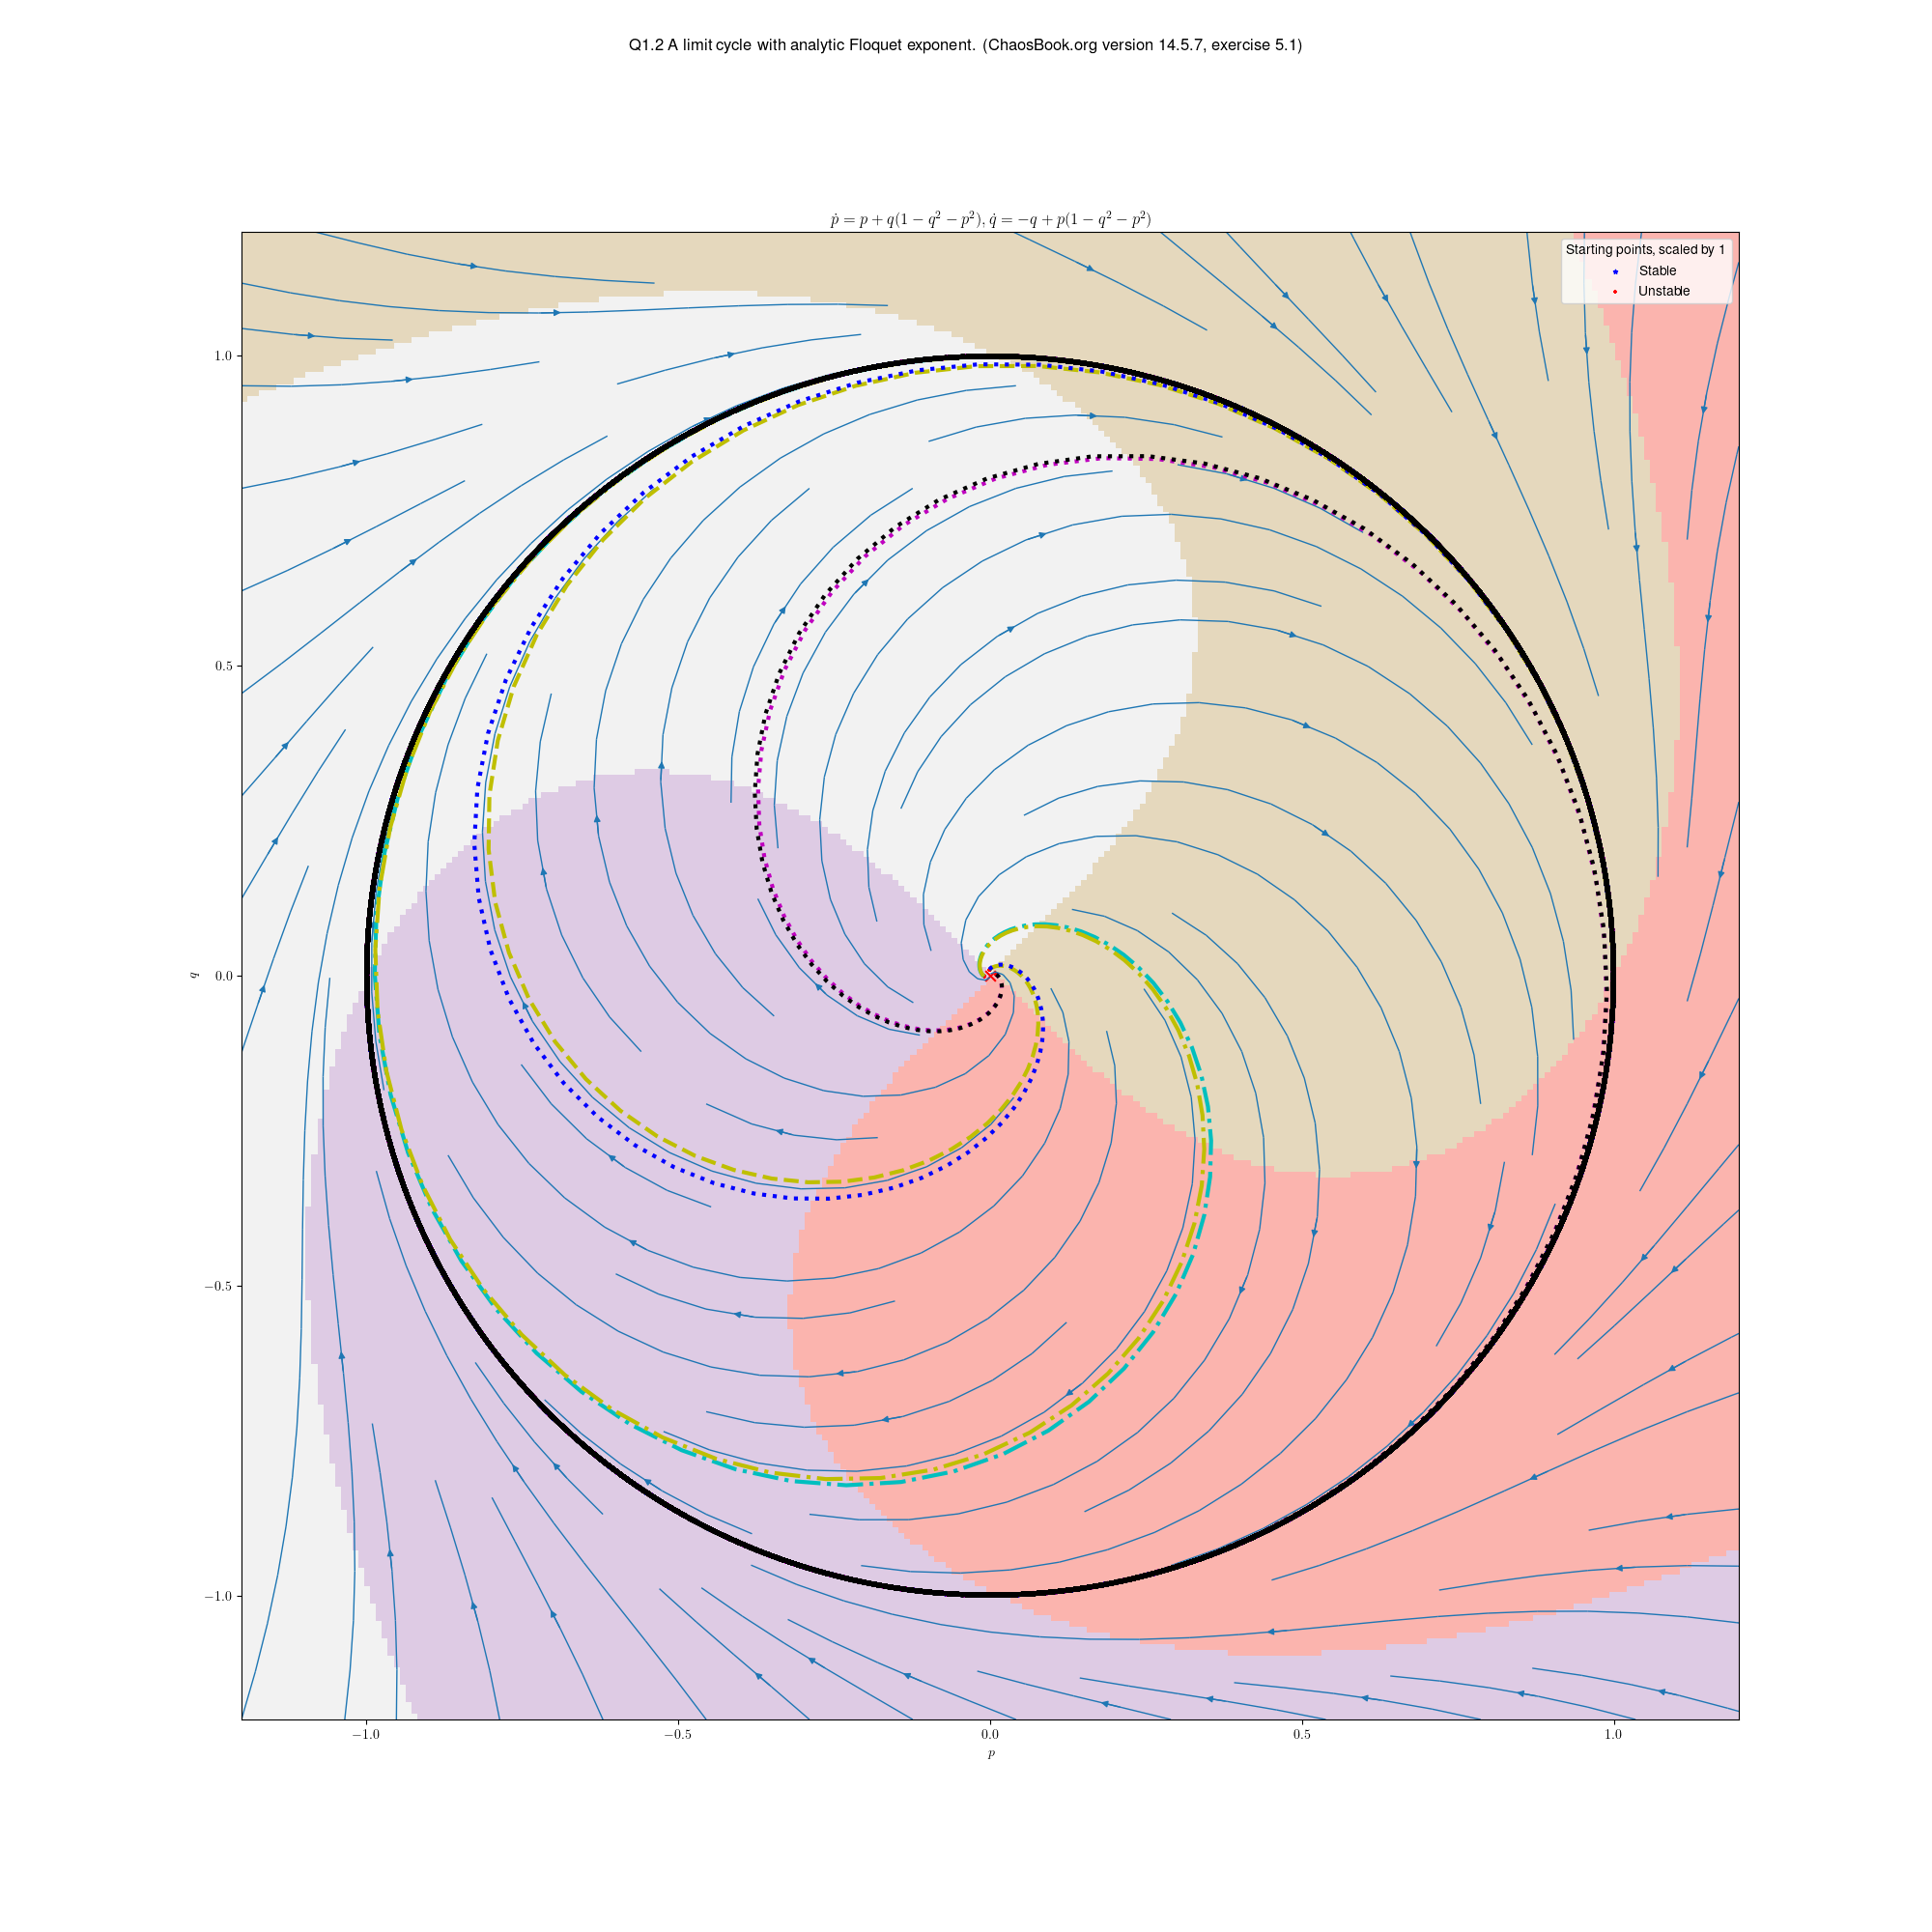
\includegraphics[width=\textwidth]{wk2/floquet.png}
\end{figure}
From \eqref{eq:dot_r0}
\begin{align*}
	\dot{r} =&	\cos{\theta} \dot{q} + \sin{\theta} \dot{p}\\
	=& 	\cos{\theta} \big[p + q\big(1-q^2-p^2\big)\big] + \sin{\theta} \big[-q + p\big(1-q^2-p^2\big)\big]\\
	=& 	\cos{\theta} \big[r \cancel{\sin{\theta}} + r \cos{\theta}\big(1-r^2\big)\big] + \sin{\theta} \big[\cancel{-r \cos{\theta}} + r \sin{\theta}\big(1-r^2\big)\big]\\
	=& r \big(1-r^2\big) \numberthis \label{eq:dot_r}
\end{align*}

Substitute $r=1+\delta r$ in \eqref{eq:dot_r}
\begin{align*}
	\dot{\delta} =& \big(1+\delta\big)\big(1 -1 -2 \delta - \delta^2\big)\\
	=& - \big(1+\delta\big) \delta (2 + \delta)\\
	\approxeq & - 2 \delta \text{, so}\\
	\delta(t) \propto & e^{-2 t}
\end{align*}
So the contracting Floquet exponent is $-2$.


\section{11}
\subsection{Exercise 11.4}
We convert  \eqref{eq:lorenz:1}, \eqref{eq:lorenz:2}, and  \eqref{eq:lorenz:2} to polar coordinates.

\begin{align*}
	x =& r \cos \theta\\
	y =& r \sin \theta \text{, we have}\\
	\dot{x} =& \dot{r} \cos \theta - r \sin\theta \; \dot{\theta}\\
	\dot{y} =& \dot{r} \sin \theta + r \cos\theta \; \dot{\theta}\\
	x\dot{x}+ y\dot{y} =& r  \dot{r} \cos^2 \theta -  \cancel{r^2 \cos \theta \sin\theta \; \dot{\theta}}+  r \dot{r} \sin^2 \theta + \cancel{ r^2 \cos\theta \sin \theta \; \dot{\theta}}\\
	=& r \dot{r} \numberthis \label{eq:rdot:1}\\
	x\dot{y}-y\dot{x}=& \cancel{r \cos \theta \dot{r} \sin \theta} +r^2 \cos^2 \theta  \; \dot{\theta} -\cancel{r \sin \theta \dot{r} \cos \theta} + r^2 \sin^2 \theta  \; \dot{\theta}\\
	=& r^2 \dot{\theta} \numberthis \label{eq:thetadot:1}
\end{align*}
Substituting  \eqref{eq:lorenz:1} and \eqref{eq:lorenz:2} in \eqref{eq:rdot:1}
\begin{align*}
	\dot r =& \frac{1}{r}\big[\sigma r^2 \cos \theta (\sin\theta-cos\theta) +  r^2 \sin \theta \big(\rho \cos\theta -sin\theta - \cos \theta z\big)\big]\\
	=& \sigma r \cos \theta \sin\theta -\sigma r \cos^2 \theta + r (\rho-z) \cos\theta \sin \theta-r \sin^2 \theta \\
	=& \big(\sigma +\rho -z \big)r \underbrace{\cos \theta \sin\theta}_\text{$\frac{\sin 2\theta}{2}$} -\sigma r \underbrace{\cos^2 \theta}_\text{$\frac{1+\cos 2\theta}{2}$}-r \underbrace{\sin^2 \theta}_\text{$\frac{1-\cos 2\theta}{2}$}\\
	=&  \big(\sigma +\rho -z \big)r \frac{\sin 2\theta}{2} - \sigma r \frac{1+\cos 2\theta}{2} -r \frac{1-\cos 2\theta}{2}\\
	=& \frac{r}{2}\big[\big(\sigma +\rho -z \big)\sin 2\theta - 1 -\sigma + \big(1-\sigma\big) \cos 2\theta\big] \numberthis \label{eq:lorenz:polar:r}
\end{align*}
Substituting  \eqref{eq:lorenz:1} and \eqref{eq:lorenz:2} in \eqref{eq:thetadot:1}
\begin{align*}
	 \dot{\theta} =& \frac{1}{r^2}\big[ r \cos \theta\big(\rho r \cos \theta -r \sin \theta - r \cos \theta z\big) - r \sigma \sin\theta \big(r \sin \theta-r \cos \theta\big) \big]\\
	  =& \cos \theta\big(\rho  \cos \theta - \sin \theta - \cos \theta z\big) -  \sigma \sin\theta \big( \sin \theta- \cos \theta\big)\\
	  =& \big(\rho-z  \big) \cos^2 \theta - \sigma \sin^2 \theta + \big( \sigma-1 \big) \cos \theta \sin \theta\\
	  =& \frac{\rho-z }{2}\big[1 + \cos 2 \theta\big] - \frac{\sigma}{2}\big[1 - \cos 2 \theta\big]+\frac{\sigma-1}{2} \sin 2 \theta\\
	  =& \frac{1}{2}\big[\rho-z -\sigma + \big(\rho-z +\sigma\big)\cos 2 \theta + \big(\sigma-1\big) \sin 2 \theta\big] \numberthis \label{eq:lorenz:polar:theta}
\end{align*}
Converting \eqref{eq:lorenz:3} to polar coordinates gives
\begin{align*}
	\dot{z} =& r^2 cos\theta \sin\theta - b z\\
	=& \frac{1}{2} r^2 \sin 2\theta -bz \numberthis \label{eq:lorenz:polar:z}
\end{align*}
Note that the transformation $\theta \rightarrow \theta + \pi$ leaves $\cos \theta$ and $\sin \theta$ unchanged, so \eqref{eq:lorenz:polar:r}, \eqref{eq:lorenz:polar:theta}, and \eqref{eq:lorenz:polar:z} are invariant.

\section{Homework 6}

\begin{align*}
	x_0 =& (0.d_1 d_2 d_3 ...)_2\\
	f(x_0) =& 2 \times \begin{cases}
		(0.0 d_2 d_3 d_4...)_2 & \text{for } d_1 = 0\\
		[1- (0.1 d_2 d_3 d_4...)_2] & \text{for } d_1 = 1
	\end{cases}\\
		=& \begin{cases}
			(0.d_2 d_3 d_4...)_2 & \text{for } d_1 = 0\\
			[0.(1-d_2) (1-d_3) (1-d_4)...]_2 & \text{for } d_1 = 1
		\end{cases}\\
	=& (0.d^\prime_2 d^\prime_3 d^\prime_4 ...)_2
\end{align*}
\section{Homework 7}
\subsection{Henon mapping}
\begin{align*}
	(x_{n+1},y_{n+1}) =& (1-ax_n^2+by_n,x_n) \numberthis \label{eq:henon:recurrence}\\
	x_n =& y_{n+1}\\
	1-ax_n^2+by_n =& x_{n+1}\\
	y_n =& \frac{x_{n+1} + a  y_{n+1}^2-1}{b}
\end{align*}
At a fixed point, \eqref{eq:henon:recurrence} becomes
\begin{align*}
	(x,y) =& (1-ax^2+by,x)\text{, ie}\\
	x =& y \text{, and}\\
	x =& 1-ax^2 +by\\
	=& 1-ax^2 +bx\text{. Gathering terms}\\
	ax^2 + (1-b)x = &1\\
	a\big[x^2 + 2\frac{1-b}{2a}x + \big(\frac{1-b}{2a}\big)^2\big]  = &1+ \frac{(1-b)^2}{2a}\\
	a\big[x+ \frac{1-b}{2a}\big]^2= &1+ \frac{(1-b)^2}{4a}\\
	\big[x+ \frac{1-b}{2a}\big]^2= &\frac{1+ \frac{(1-b)^2}{4a}}{a}\\
	x = - \frac{1-b}{2a} \pm \sqrt{\frac{1+ \frac{(1-b)^2}{4a}}{a}}
\end{align*}
\bibliographystyle{unsrt}
\addcontentsline{toc}{section}{Bibliography}
\bibliography{../dynamics}

\end{document}
